\subsection{L'objet PROPERTY (propriété)}
\label{subsec:property}
L'objet \lstinline{PROPERTY} est un outil proposé par CodeSys pour la programmation orientée objet. Il permet de définir des attributs (variables) propres à un contexte avec un niveau d'accessibilité paramétrable (publique, privée, protégée ou interne).

Cela signifie que l'on peut définir des variables à l'intérieur d'une classe qui pourront être accessibles depuis l'extérieur de la classe par l'intermédiaire de méthodes appelées \emph{accesseurs}.

\begin{UPSTIinfor}{Les accesseurs}
    Il existe deux types d'accesseurs : GET et SET. 
    \begin{description}
        \item[GET] : Permet de lire la valeur d'une variable
        \item[SET] : Permet d'écrire la valeur d'une variable
    \end{description}
    \begin{minipage}{.45\linewidth}
        \begin{lstlisting}
            C<ClassName>.<propertyName>.Get 
                <propertyName> := THIS^.m_<localName>;
        \end{lstlisting}
    \end{minipage}%
    \hfill
    \begin{minipage}{.45\linewidth}
        \begin{lstlisting}
            C<ClassName>.<propertyName>.Set 
                THIS^.m_<localName> := <propertyName>;
        \end{lstlisting}
    \end{minipage}

    Il est possible de supprimer un des accesseurs pour rendre la propriété en lecture seule ou en écriture seule.

    Lors d'une dérivation, les propriétés de la classe sont héritées et leurs accesseurs peuvent être surchargés.
\end{UPSTIinfor}

Une propriété est donc un objet que l'on associe à une POU. On décrit ensuite ses accesseurs pour définir comment lire ou écrire la valeur de la propriété.
Ce sont elles qui permettent d'obtenir une encapsulation des données. En effet, elles permettent de contrôler l'accès aux données de l'objet (variables internes, d'un POU, d'un BF ou d'une variable globale -- GVL). Elles agissent comme un filtre ou une surchage. 


\begin{UPSTIinfor}{Ajout d'un propriété sous CodeSys}
    \begin{minipage}{.7\linewidth}
        Sous CodeSys, les propriétés et les méthodes sont ajoutés à la POU en utilisant l'outil \emph{Add Object}. Il suffit alors de sélectionner le type de l'objet à ajouter (propriété ou méthode) et de le nommer.
    \end{minipage}\hfill
    \begin{minipage}{.2\linewidth}
        \centering
        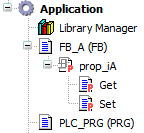
\includegraphics[width=\linewidth]{_cds_img_property.png}
    \end{minipage}    
\end{UPSTIinfor}

\begin{UPSTIidee}{Propriétés de la classe CStep}
    Par exemple, si notre classe \emph{CStep} possède un attribut \emph{m\_xActivityBit}, nous allons ajouter une propriété \emph{xActivityBit} à notre bloc fonctionnel \emph{FB\_CStep}. Cette propriété, en lecture seule, n'aura pas d'accesseur \emph{SET}. Son accesseur \emph{GET} sera défini de la manière suivante :
    \begin{lstlisting}
FB_CStep.xActivityBit.Get
    xActivityBit := THIS^.m_xActivityBit;
    \end{lstlisting}
\end{UPSTIidee}

\begin{UPSTIinfor}{Les attributs d'accessibilité}
    Les méthodes et les attributs sont associées à un attribut d'accessibilité. Cela permet de contrôler l'accès aux méthodes et aux attributs de la classe : 
    \begin{description}
        \item[PRIVATE] : Accessibilité réduite à l'entité à laquelle elle est associée.
        \item[PROTECTED] : Accessibilité réduite à l'entité à laquelle elle est associée et à ses dérivées.
        \item[PUBLIC] : Accessibilité à toutes les entités.
        \item[INTERNAL] : Accessibilité réduite à l'espace de noms de la bibliothèque
    \end{description}
\end{UPSTIinfor}
